\documentclass[xcolor=dvipsnames,11 pt]{beamer}

\usepackage{amssymb,amsfonts}
\usepackage{amsmath}
\usepackage{booktabs}
\usepackage{lmodern}
\usepackage{graphicx}
\usepackage{tikz}
\usepackage{verbatim}

\usefonttheme[onlymath]{serif}
\setbeamerfont{frametitle}{size=\large, shape=\normalfont}
\vfuzz=25pt
\hbadness=10000
\vbadness=10000

\usetheme{Copenhagen}
\usecolortheme[RGB={240,160,40}]{structure}
\setbeamertemplate{navigation symbols}{}
\setbeamertemplate{footline}[frame number]

\title{Random Graphs and Applications}
\author{{\bf N.R.Aravind}}
\date{}

\begin{document}

\maketitle

\frame
{
\frametitle{Triangle-free graphs}

\begin{center}
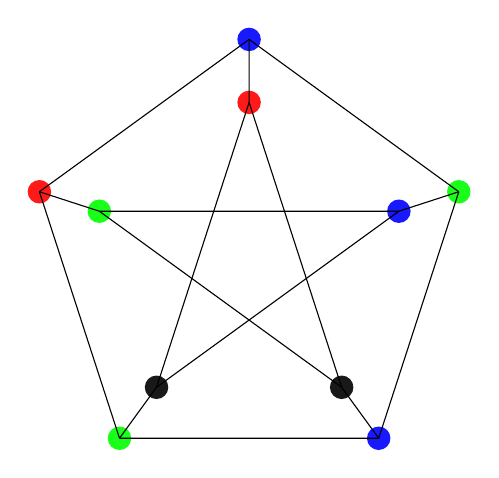
\begin{tikzpicture}[scale=.8,rotate=18,auto=center,every node/.style={circle,inner sep=3pt}]
\draw (0*360/5: 2.5cm) node[fill=blue!90]{};
\draw (1*360/5: 2.5cm) node[fill=red!90]{};
\draw (2*360/5: 2.5cm) node[fill=green!90]{};
\draw (3*360/5: 2.5cm) node[fill=black!90]{};
\draw (4*360/5: 2.5cm) node[fill=black!90]{};

\foreach \a/\b in {0/144,0/216,72/216, 72/288,144/288}{
\draw (\a: 2.5cm) -- (\b: 2.5cm);}

\draw (0*360/5: 3.5cm) node[fill=green!90]{};
\draw (1*360/5: 3.5cm) node[fill=blue!90]{};
\draw (2*360/5: 3.5cm) node[fill=red!90]{};
\draw (3*360/5: 3.5cm) node[fill=green!90]{};
\draw (4*360/5: 3.5cm) node[fill=blue!90]{};

\foreach \a/\b in {0/72,72/144,144/216,216/288,288/0}{
\draw (\a: 3.5cm) -- (\b: 3.5cm);}


\foreach \a in {0,72,144,216,288}{
\draw (\a: 2.5cm) -- (\a: 3.5cm);}

\end{tikzpicture}
\end{center}
}

\frame
{
\frametitle{Nodes in a grid}
\begin{center}
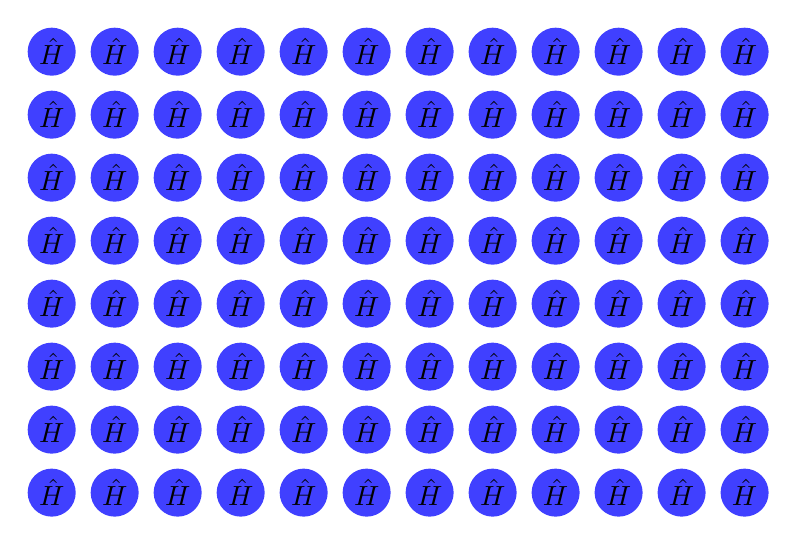
\begin{tikzpicture}[scale=.8,auto=center,every node/.style={circle,inner sep=1.5pt}]
 \foreach \x in {0,...,11}
    \foreach \y in {0,...,7}
      \node[fill=blue!75] at (\x,\y){$\hat{H}$} ;
\end{tikzpicture}
\end{center}
}

\end{document}
